\section{DevOps}
DevOps ist eine Philosophie oder Organisationsform, mit der Continuous Delivery optimal funktioniert. Es stellt dabei eine Kollaboration zwischen Entwicklung (Developement) und Betrieb (Operations) in den Mittelpunkt, wodurch bereits das Wesentliche des Gedankens hervorgeht: Ein Zusammenwachsen der beiden Abteilungen zu einem Verband (siehe Abbildung \ref{fig:devops}). In klassischen Organisationsformen sind diese in mindestens zwei unterschiedliche Abteilungen getrennt und verfolgen verschiedene Ziele. Während bei dem Betrieb Kosteneffizienz in den Vordergrund rückt, stellt die Entwicklung neue Features bereit und wird an der Geschwindigkeit und Effizienz ihres Vorgehens gemessen. Bei der Einführung von Continuous Delivery sollten Betrieb und Entwicklung daher zusammenarbeiten, um das Notwendige Wissen und entsprechende Werkzeuge zu teilen. Jede Gruppe beherrscht durch die unterschiedliche Perspektive auf die Anwendungen einen Teil von Continuous Delivery besonders gut. Der Betrieb kennt beispielsweise Aspekte wie Monitoring, Security oder Netzinfrastrukturen. Ohne diese kann eine Anwendung kaum sinnvoll installiert oder betrieben werden kann. Die Entwicklung hingegen kennt den Code, die Entwicklungsinfrastruktur und Middleware wie Application Server etc. sehr genau. Gemeinsam lässt sich somit eine Continuous-Delivery-Pipeline aufbauen. Mit der Einführung von Continuous Delivery sollte allerdings auch die Einführung von DevOps in Betracht gezogen werden [1].\\ \\
Bereits 2006 wurde bekannt, dass eines der großen IT-Unternehmen einen anderen Ansatz zur Erstellung seiner Dienste verfolgt. Die Trennung von Betrieb und Entwicklung wurde bis dato von allen IT-Organisationen umgesetzt. Zu diesem Zeitpunkt gab es bei Amazon bereits Teams, die sowohl die Entwicklung als auch den Betrieb vereinen. Jedes Team ist somit für eine spezifische Fachlichkeit zuständig und kann diese unabhängig von anderen Teams als Service implementieren. Der Dienst kann schließlich selbständig optimiert werden, um einen guten Betrieb zu ermöglichen. Des Weiteren kann ohne weitere Abstimmung eine Weiterentwicklung am Dienst vorgenommen werden. Auch der eingesetzte Technologie-Stack ist abhängig von der Entscheidung des Teams. Diese übernehmen die vollständige Verantwortung für ihre Komponenten. Daraus folgt eine geringere Koordination untereinander, wodurch wiederum Software schneller entwickelt und in Produktion gebracht werden kann. Auch Kunden wissen direkt, welcher Ansprechpartner für welchen Service zuständig ist (siehe Abbildung \ref{fig:devops}) [1].\\ \\
Continuous Delivery wird häufig auch mit DevOps gleichgesetzt. Das trifft jedoch nicht zu. Durch DevOps lässt sich Continuous Delivery zwar drastisch vereinfachen, allerdings gibt es neben dieser (wesentlichen) Praktik im DevOps-Umfeld noch weitere Bereiche (Monitoring, Troubleshooting etc.), bei denen diese Organisationsform und eine damit einhergehende Zusammenarbeit sinnvoll sein kann [1].\\
\begin{figure*}[h!]
	\centering
	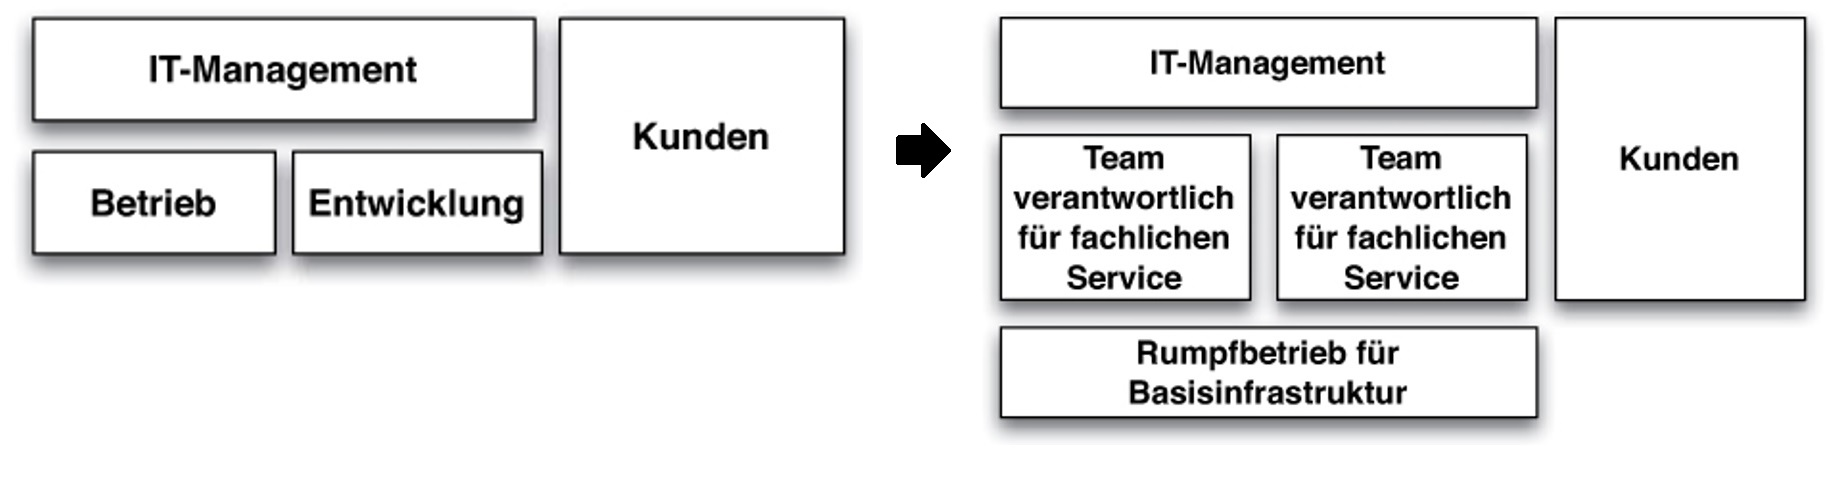
\includegraphics[width=0.8\linewidth]{images/devops}
	\caption{Wandel von klassischer Organisation zu DevOps-Teams} %Generelle
	\label{fig:devops}
\end{figure*}
